% !TEX encoding = UTF-8 Unicode
\documentclass[a4paper]{article}

\usepackage{color}
\usepackage{url}
\usepackage{xurl}
\usepackage[T2A]{fontenc} % enable Cyrillic fonts
\usepackage[utf8]{inputenc} % make weird characters work
\usepackage{wrapfig}
\usepackage{graphicx}

\usepackage[english,serbian]{babel}
%\usepackage[english,serbianc]{babel} %ukljuciti babel sa ovim opcijama, umesto gornjim, ukoliko se koristi cirilica

\usepackage[unicode]{hyperref}
\hypersetup{colorlinks,citecolor=green,filecolor=green,linkcolor=blue,urlcolor=blue}

\usepackage{listings}

%\newtheorem{primer}{Пример}[section] %ćirilični primer
\newtheorem{primer}{Primer}[section]

\definecolor{mygreen}{rgb}{0,0.6,0}
\definecolor{mygray}{rgb}{0.5,0.5,0.5}
\definecolor{mymauve}{rgb}{0.58,0,0.82}

\lstset{ 
  backgroundcolor=\color{white},   % choose the background color; you must add \usepackage{color} or \usepackage{xcolor}; should come as last argument
  basicstyle=\scriptsize\ttfamily,        % the size of the fonts that are used for the code
  breakatwhitespace=false,         % sets if automatic breaks should only happen at whitespace
  breaklines=true,                 % sets automatic line breaking
  captionpos=b,                    % sets the caption-position to bottom
  commentstyle=\color{mygreen},    % comment style
  deletekeywords={...},            % if you want to delete keywords from the given language
  escapeinside={\%*}{*)},          % if you want to add LaTeX within your code
  extendedchars=true,              % lets you use non-ASCII characters; for 8-bits encodings only, does not work with UTF-8
  firstnumber=1000,                % start line enumeration with line 1000
  frame=single,	                   % adds a frame around the code
  keepspaces=true,                 % keeps spaces in text, useful for keeping indentation of code (possibly needs columns=flexible)
  keywordstyle=\color{blue},       % keyword style
  language=Python,                 % the language of the code
  morekeywords={*,...},            % if you want to add more keywords to the set
  numbers=left,                    % where to put the line-numbers; possible values are (none, left, right)
  numbersep=5pt,                   % how far the line-numbers are from the code
  numberstyle=\tiny\color{mygray}, % the style that is used for the line-numbers
  rulecolor=\color{black},         % if not set, the frame-color may be changed on line-breaks within not-black text (e.g. comments (green here))
  showspaces=false,                % show spaces everywhere adding particular underscores; it overrides 'showstringspaces'
  showstringspaces=false,          % underline spaces within strings only
  showtabs=false,                  % show tabs within strings adding particular underscores
  stepnumber=2,                    % the step between two line-numbers. If it's 1, each line will be numbered
  stringstyle=\color{mymauve},     % string literal style
  tabsize=2,	                   % sets default tabsize to 2 spaces
  title=\lstname                   % show the filename of files included with \lstinputlisting; also try caption instead of title
}

\begin{document}

\title{Problemi rodne ravnopravnosti u informatici u svetu\\ \small{Seminarski rad u okviru kursa\\Metodologija stručnog i naučnog rada\\ Matematički fakultet}}

\author{Andrijana Aleksić, Bogdan Marković, Jelena Keljać, Luka Jovičić\\annaleksic95@gmail.com, bogdanis799@gmail.com,\\jelena.keljac9@gmail.com, luka.jovicic16@gmail.com}

%\date{9.~april 2015.}

\maketitle

\abstract{U ovom radu prikazujemo istorijski osvrt na temu rodne ravnopravnosti u informatici i opis trenutnog stanja u ovoj oblasti: iako je ovo oblast kojom su nekada dominirale žene, to je danas značajno drugačije. Izlažemo pregled literature koja objašnjava ovaj problem, počev od obrazovnog sistema, pa do poslodavaca u industriji ili akademiji. Na kratko se osvrćemo na stanje u Srbiji i poredimo je sa situacijom u svetu. Za kraj, ističemo nekoliko inicijativa koje se bave rodnom ravnopravnošću u informatici i njihove ciljeve, metode i rezultate koji nas dovode do ravnopravnijeg društva, što će koristiti svima.}

\tableofcontents

\newpage

\section{Uvod}
\label{sec:uvod}
Proteklih godina pratimo ubrzan razvoj IT industrije, kako u svetu, tako i u Srbiji. Sve veći broj mladih odlučuje se za prestižne fakultete u svetu informatike i matematike. Da li ovaj razvoj prate podjednako žene i muškarci? Da li oba pola imaju jednake mogućnosti, plate, pružene prilike? Potvrdan odgovor na oba pitanja je ključan kako bi se obezbedila rodna ravnopravnost u IT-ju.

Zašto postoji veliki jaz u procentu žena u IT industriji u odnosu na muškarce? Da li se radi na ovome i kojim metodama? Pokazuje se da poslednjih godina broj žena jeste u porastu. Naime, sve veći broj studentkinja se opredeljuje za smerove informatike, iako se na osnovu statistika primećuje da još uvek ne postoji ravnopravnost.

\section{Rodna ravnopravnost kroz istoriju}
\label{sec:istorija}
Iako se danas na osnovu dostupne statistike može zaključiti da je informatika prvenstveno ,,muška'' oblast, istorijski gledano, situacija je bila drugačija. Same početke informatike i računarskih nauka obeležile su žene. Mnoge od njih nepravedno su zaboravljene, te se zato danas stiče utisak da se odnos polova u informatici nije menjao kroz vreme.

Ada King Lavlejs (1815-1852), ćerka čuvenog engleskog pesnika Džordža Gordona Bajrona, smatra se prvom osobom koja se bavila programiranjem. Već sa 17 godina upoznala je Čarlsa Bebidža, zajedno sa kojim je radila na nacrtu za diferencijalnu mašinu, kao i za analitičku mašinu za koju je napisala prvi algoritam \cite{brockwell}. Pisala je o Bebidžovom radu gde je predlagala svoje ideje i unapređenja, ističući da ,,računar može da uradi bilo šta što može biti logički uočeno''. Nažalost, preminula je sa samo 36 godina života, te nikad nisu konstruisali mašinu \cite{davis}. Pored toga, ostavila je ogroman trag u razvoju informatike i postala poznata i kao ,,majka programiranja''. Njeni i Bebidževi zapisi korišćeni su za konstruisanje prvog računara čak oko 100 godina kasnije \cite{npr, fuegi}.

Nakon Američkog građanskog rata, žene su zapošljavane kao ,,ljudski računari'', i to najčešće udovice, dok su ostale dobijale priliku kada je falilo muške radne snage. Bile su manje plaćene nego muškarci, dok su neke čak i volontirale, iako su bile jednako sposobne \cite{evans}. Dodatno, većina poslova koje su žene obavljale, školovani muškarci smatrali su nezanimljivim ili nedovoljno plaćenim. Vremenom su žene počele i da se školuju za računarske poslove, te je njihov broj u ovoj oblasti neprestano rastao \cite{sobel}.

{\sloppy
Tokom Prvog svetskog rata, s obzirom na veliki broj mu\-ška\-raca koji su bili na bojnom polju, većina računarskih poslova pripala je ženama. U Velikoj Britaniji vršile su složena izračunavanja, koja su pomogla Britaniji tokom rata. Nakon toga su samo neke uspevale da opstanu kao profesori u srednjim školama, dok je većina ostala bez posla \cite{grier}. Muški školovani inženjeri gledali su na ta neophodna izračunavanja kao na poslove nedostojne njihove ekspertize, jer je ovaj posao smatran činovničkim. Taj trend nastavio se i tokom i nakon Drugog svetskog rata.}

Pored činjenice da je na ENIAC-u, jednom od prvih elektronskih raču\-nara, radilo 6 žena (,,ENIAC žene''), koje se danas proslavljaju kao prve programerke u modernom smislu reči, tada njihov uticaj nije cenjen koliko je zasluženo. Muški inženjeri mahom su bili koncentrisani na hardver, te su razvoj softvera smatrali manje prestižnom oblašću \cite{frink}. Koliko je samo programiranje softvera i uticaj žena bio zanemaren, pokazuje činjenica da su tadašnji mediji u vreme predstavljanja ENIAC-a potpuno zanemarili imena žena koje su učestvovale u projektu \cite{npr}.

Sličan tim programerki je zatim radio na UNIVAC-u (jednom od prvih komercijalnih računara) zajedno sa Grejs Hoper, čuvenom profesorkom matematike i jednom od pionira modernog programiranja. Od nje je potekla ideja da se računarski programi pišu engleskim jezikom, a ne pomoću brojeva, kako su se do tada pisali. Tako je nastao prvi kompajler. Na taj način je uticala da se softver po svojoj značajnosti izjednači sa hardverom, ako ne i da postane bitniji. Sa engleskog jezika program je mogao da se prevodi za bilo koji željeni hardver \cite{npr}. Međutim, iako se status hardvera poboljšao, ovo nije pozitivno uticalo na broj žena u informatici.

Kako je značajnost programiranja postajala sve jasnija, poslodavci su počeli da traže mlade muškarce zainteresovane za računare. Protiv žena su se povremeno vodile i kampanje sa ciljem da se programiranje promoviše kao dominantno muška oblast. ,,Šta ima 16 nogu, 8 brzih jezika i košta te barem 40 000 dolara godišnje?'' bio je samo jedan od naslova. Čak ni Kosmopolitanov članak ,,Devojke računarstva'' nije pomogao da se ovakav trend spreči. Odjednom je programiranje postajalo prestižna i cenjena oblast. Zato su krajem šezdesetih godina prošlog veka nastupile velike promene u odnosu polova u programiranju. Broj žena je i dalje bio značajan, ali su bile znatno manje plaćene \cite{evans, frink}.

{\sloppy
Tokom narednih godina, polako se uspostavljala dominacija broja mu\-ška\-raca u ovom odnosu. Prema nekim autorima, testovi koje su dobijali kandidati za posao bili su namerno više prilagođeni muškarcima \cite{frink}, kreirane su video igre pune akcije tako da su primarno ciljale muškarce koji su činili većinu korisnika računara. Broj žena u računarstvu dostigao je vrhunac sredinom 1984. godine kada je procenat ženskih diplomaca bio 37.1\%. Zatim je usledio konstantan pad, gde je već 1998. taj broj bio 26.7\% \cite{camp}.}

U 21. veku situacija se nije mnogo menjala, te je od početka veka procenat ženskih diplomaca konstatno ispod 20\%. Pokrenut je veliki broj inicijativa i uložena ogromna količina novca sa ciljem da se među devojčicama i adolescentkinjama promovišu računarske nauke, sa ciljem da se jaz među polovima umanji \cite{aei}. Takođe je zastupljeniji naučni rad u ovoj oblasti, sa više konferencija i časopisa koji su posvećeni isključivo problemima rodne ravnopravnosti u informatici i uopšte u MINT disciplinama (matematika, inženjerstvo, nauka i tehnologija, od eng. \emph{STEM}) \cite{soe-yakura}.

Veliki broj istraživača ovog odnosa kroz istoriju smatrao je da su relevantni uzori jedan od glavnih faktora koji utiče na to da li će se mlade devojke odlučiti za programiranje. S obzirom da istorija nepravedno zanemaruje trag koji su žene ostavile u programiranju, posebno u samim počecima, broj istorijskih uzora nije veliki. Međutim, postavlja se pitanje da li je to zaista presudno, i koji su sve faktori koji utiču na tako veliki jaz među polovima? U svakom slučaju, ako se na osnovu istorije nešto može zaključiti, to je da nema opravdanja da se informatika smatra profesijom predodređenom za bilo koji od polova, bez obzira na statističke podatke.
% \input{chapters/2_obrazovanje}
\section{Odnos polova u informatici u svetu}
\interfootnotelinepenalty=10000
\label{sec:usvetu}
Postoji širok konsenzus da su žene manje zastupljeni pol u informatici: prema podacima Eurostata, one čine 18.5\% IKT stručnjaka u Evropskoj Uniji,\cite{gendergap-eu} prema izveštaju britanskog \emph{Tech Nation}-a u Ujedinjenom Kraljevstvu ovaj broj je 19\%,\cite{gendergap-uk} a američki Nacionalni centar za žene i informacionu tehnologiju je 2016. objavio da tek 26\% poslova vezanih za računarstvo obavljaju žene i to prvenstveno na pozicijama projektne menadžerke i biznis analitičarke (dok su muškarci češće softverski inžinjeri i sistem administratori) \cite{gendergap-us}. Još gora situacija je na rukovodećim pozicijama, što se može videti na slici \ref{fig:rukovodece}.

\begin{figure}[h!]
\begin{center}
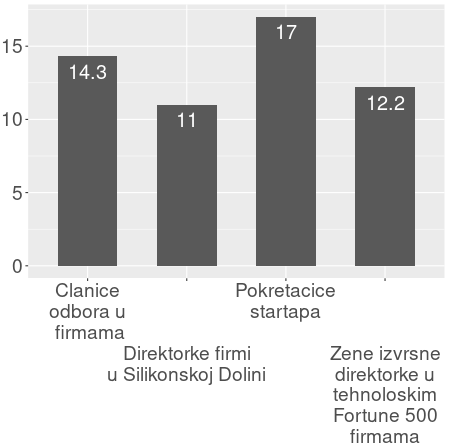
\includegraphics[width=6cm, height=5cm]{zene-na-rukovodecim-pozicijama.png}
\end{center}
\caption{Procenat žena na rukovodećim pozicijama \cite{leadership-women}. Na x osi se nalazi naziv pozicije, a na y procenat žena na toj poziciji.}
\label{fig:rukovodece}
\end{figure}

U ovom odeljku ćemo dati pregled literature s ciljem da čitaoca upoznamo sa položajem žena u informatici i razlozima zašto je on takav. Pošto u literaturi često ne postoje precizniji termini, koristićemo srodne oblasti u prezentaciji podataka i zaključaka. Tako ćemo kada pričamo o Evropi uglavnom posmatrati blisku oblast informacionih i komunikacionih tehnologija (IKT), a u Americi ćemo se češće susretati sa nešto širom grupom već pomenutih MINT oblasti.

\subsection{Obrazovanje i analogija bušne cevi}
Jedno od popularnijih objašnjenja za činjenicu da su žene manje zastupljene u MINT poslovima u odnosu na relevantne obrazovne smerove u preduniverzitetskom i univerzitetkom obrazovanju je preko analogije ,,bušne cevi'': iako je na početnim stupnjevima odnos polova ujednačeniji, učenice i studentkinje neproporcionalno više odustaju na svakom koraku svog obrazovnog puta \cite{jacobs, soe-yakura, blickenstaff}. Međutim, ova analogija nije opšteprihvaćena. Leventman primećuje da postoje tri načina pomoću kojih se može doći do karijere u informatici: tradicionalni, nakon višeg obrazovanja, zatim tranzicioni, ako zaposlena dolazi iz druge oblasti, i samousmereni tj. samouki \cite{leventman}. Ovo znači da osim ,,curenja'' postoji i obrnut proces, ,,ubrizgavanje''. Bartol i Esprej navodne konkretan primer Sjedinjenih država 1996. godine, kada se broj poslova povećao za 200000, a broj dodeljenih diploma u informatičkim disciplinama je bio svega 45000 na svim stepenima studija \cite{bartol}.

So i Jakura analogiju cevi odbacuju kao prejednostavnu, te da umesto traženja rešenja za probleme u jednoj ili par faza u obrazovanju ili zapošljavanju (npr. fokusiranje samo na fakultet ili zapošljavanje), problem treba posmatrati iz dublje kulturološke perspektive. One takođe tvrde da nije dovoljno imati samo nekoliko pojedinaca koji bi rešavali problem ili bili primer, već je neophodno ostvariti kritičnu masu žena i/ili muškaraca, na vodećim pozicijama koji bi razumeli i adekvatno adresirali sve probleme koji dovode do neravnopravnosti na nivou celokupne zajednice \cite{soe-yakura}.

\subsection{Razlozi za nejednaku zastupljenost} 
Postoji nekoliko različitih grupa teorija zašto su žene manje zastupljen pol. Najjednostavnija krivicu pripisuju nedostatku sposobnosti devojčica i žena: Bares ovo naziva ,,hipotezom Lerija Samersa'' po bivšem predseniku Harvarda i opisuje kao krivljenje žrtve \cite{barres}. Samers je jednom prilikom izjavio da su glavni razlozi manje zastupljenosti žena u inženjerskim disciplinama genetske predispozicije i lični izbori; ovo je izazvalo velika negodovanja u naučnoj zajednici i tvrdnje da su njihova istraživanja pogrešno interpretirana, a Samers se kasnije izvinio zbog svojih reči \cite{lawler}.

Druga grupa pretpostavlja da je u pitanju njihov izbor prouzrokovan različitim okolnostima\cite{hellens, blickenstaff}. Blikenstaf odbacuje biološke razlike i nudi jednu sistematizaciju razloga zašto devojčice češće odustaju od karijere u MINT oblastima: u manjoj meri nedostatak pozitivnih iskustava devojčica sa naukom i averzija prema relevantnim predmetima, nedostatak ženskih uzora i neadekvatni kurikulumi, a značajnije neadekvatan pedagoški pristup nastavnika, klima u kojoj se favorizuju i više se očekuje od dečaka i muški pogled na svet koji dominira u nauci \cite{blickenstaff}. Treća grupa objašnjenja se fokusira na prepreke na koje žene nailaze u svom akademskom i karijernom putu: Svaford i kolege kao neke od faktora koji sputavaju žene u MINT karijerama navode seksizam i postojanje ,,staklenog plafona'' za žene u ovim poslovima \cite{swafford}.

Kada je reč o zaposlenju, Vin i Korel su ispitivale kako se predstavnici tehnoloških kompanija odnose prema potencijalnim kandidatima, studentima završnih godina na jednom američkom univerzitetu koji su izrazili interesovanje za poziciju u kompanijama. One su primetile da su već u inicijalnom koraku pri zapošljavanju zastupljene razne prakse koje su diskriminatorne prema ženama. Ističu da je tipično da muškarci dominiraju u vodećim ulogama na intervjuima, dok su žene često marginalizovane ili su zadužene samo za netehničke delove. Takođe su učestale reference na štrebersku (eng. \emph{geek}) kulturu, koja je po prirodi maskulina, kao i propagiranje rodnih stereotipa, što ima veliki potencijal da odbije ženske kandidate u startu. Manje startap firme su posebno odgovorne za deljenje poklona koji mogu biti uvredljivi ženama, poput majici s natpisima \emph{'I like big data and I cannot lie'} (referenca na pesmu \emph{Sir Mix-A-Lot}-a iz 1992), \emph{'I’ll show you my data if you show me yours.'} i \emph{'Finding your faults, just like mom'} \cite{wynn}. Startapi i startap kultura se često karakterišu kao seksističke, a ove firme iako pojedinačno male, čine nezanemarljiv deo poslodavaca \cite{steinberg-forbes}.

U jednom od istraživanja koje se fokusiralo na radnu populaciju, Levelin i kolege su sproveli istraživanje nad alumnijima \emph{Georgia Tech}-a koji su se u međuvremenu zaposlili, s ciljem da saznaju više o karijernim putevima žena i manjinskim grupama u IT sektoru. Jedan od rezultata, koji se fokusira na iskustva na poslu, je da žene značajno češće kažu da su diskriminisane na poslu i da su značajno manje zadovoljne benefitima (obe skale su nastale agregiranjem više relevantnih stavki koje međusobno koreliraju, tj. istraživači prezentovali rezultate kroz kompozitne mere) \cite{llewellyn}.

Evidentna je i razlika u plati, pa tako žene u tehnološkom sektoru u Sjedinjenim Državama primaju u proseku 8600 dolara godišnje manje od njihovih muških kolega, a razlika između polova postoji čak i kada se uzmu u obzir i drugi faktori poput iskustva, pozicije, lokacije i obrazovanja \cite{dhi}. Segovia-Perez i koleginice su analizirale podatke za Španiju i zaključile da ova razlika procentualno raste kako se povećavaju plate, što ukazuje na diskriminaciju prema ženama, posebno na višim pozicijama \cite{segovia}.

Iako smo se do sad fokusirali na Evropu i Ameriku, važno je napomenuti da slična iskustva žena i odnosi između polova u informatici nisu univerzalna. Recimo, u Maleziji su žene dominantan pol na IKT studijama, a iako ne postoji precizna statistika o zastupljenosti polova prema oblasti zaposlenja, postoji razlog da se veruje da žene nisu manje zastupljen pol u IKT ni nakon studija. Melstrom u svom radu izlaže detaljnu analizu ove pojave i sagledava rodne, ali i istorijske, etničke i kulturološke specifičnosti Malezije i konkretne intervencije u informatičkom obrazovanju i predlaže sličan pristup za druge države  \cite{mellstrom}. Zaključci iz ovog istraživanja se teško mogu generalizovati, ali nas podsećaju da je drugačija realnost moguća kao rezultat pažljivo odabranih intervencija i politika.

Još jedna zanimljiva pojava je paradoks jednakosti polova u MINT oblastima: Stoet i Giri su pronašli direktnu korelaciju između rodne egalitarnosti i manje zastupljenosti žena na MINT studijama, suprotno od onoga što je intuitivno očekivano \cite{stoet}. Međutim, ovo istraživanje je postalo kontroverzno kada Ričardson i kolege\cite{richardson} nisu uspeli da reprodukuju ove rezultate, a ni u ispravci originalnog nisu promenjeni zaključi. Ova rasprava nije dobila epilog i ne postoji širi naučni konsenzus o ovome \cite{schleunes-scientist}.
\subsection{Razlika između akademije i industrije}
Zastupljenost istraživačica u tehnološkim i inženjerskim oblastima u višem obrazovanju u Evropi varira, od 14.94\% u Luksemburgu i 15.73\% na Malti, do 39.3\% u Crnoj Gori i 44.4\% u Rumuniji, prema podacima Evropske Unije za 2017. godinu \cite{shefigures}. S obzirom da nisu sve zemlje učestvovale u ovom istraživanju svake godine, teško je doći do verodostojne vrednosti proseka, ali je bezbedno reći da je on nešto povoljniji za žene nego zbirne brojke date na početku ovog poglavlja.\footnote{Zainteresovani čitalac može pronaći podatke u interaktivnom obliku na portalu Evropske kancelarije za publikacije na adresi \url{https://quantos-stat.shinyapps.io/GUI_SF/}. U meniju s leve strane odabrati \emph{Chapter 4}, indikator \emph{Proportion (\%) of women among researchers}, jedinicu \emph{HC} (headcount), sektor \emph{HES} (higher education) i polje \emph{Engineering and technology}.} S obzirom na ovoliki raspon, nije moguće generalizovati bilo koji konkretan zaključak na ceo kontinent, posebno pošto postoje države u kojima je situacija skoro ravnopravna.

U Sjedinjenim Američkim Državama, situacija je obrnuta: u akademiji se računarskim naukama bavi svega 15\% žena \cite{way}. Neke od razloga zašto je razlika u polovima ovde veća možemo potražiti u činjenici da je razlika u plati izraženija u akademiji (i to za 50\% u odnosu na industriju, prema istraživanju koje su sproveli Ding i kolege \cite{ding}) i da je akademska karijera dosta nepovoljnija po (buduće) majke, s obzirom da su u SAD trudnički i porodiljski benefiti (uključujući i karijerni put novih roditelja) bolji u industriji \cite{morgan}. Ovi razlozi u opštem slučaju ne važe za Evropu.
\section{Rodna ravnopravnost u informatici u Srbiji}
\label{sec:usrbiji}
Od 1489 prijavljenih za program ,,Prekvalifikacije za IT'' u organizaciji kabineta predsednice Vlade Srbije, 55\% su žene. U okviru programa ,,Škole za 21. vek'', British Council je razvio vodič i niz aktivnosti kako bi pomogao osnovnim školama da osnuju sekcije za programiranje kao vannastavnu aktivnost. Ovaj program pohađaju podjednako devojčice i dečaci, što je indikator da iako su istorijski žene u Srbiji činile svega 20 do 30\% IT industrije, broj je u porastu \cite{veb1}. Ukoliko se osvrnemo na podatke iz naše okoline, vidimo da je sve veći broj studentkinja koje se prijavljuju za tehničke i prirodno-matematičke fakultete, ali su devojke i dalje u manjini. 

Majkrosoft Razvojni Centar u Srbiji je pokrenuo zanimljivu inicijativu pod nazivom \emph{Women know IT}. Grupa već uspešnih žena iz IT industrije, bilo da su to softverske inženjerke ili žene iz \emph{HR}-a, odlučile su da naprave pokret koji će pozivati sve više mladih devojaka da vide pogodnosti ovog posla, da se ohrabre da krenu putem IT-a iako trenutno deluje da je to muški posao zbog ogromne razlike u procentu muškaraca u odnosu na žene u ovoj industriji. Pokrenute su pre svega jednodnevne radionice u kojima se provodi dan sa studentkinjama ili devojkama koje su u srednjim školama. U toku tog dana, postoje diskusije o poslu, pogodnostima, mogućnostima napredovanja. Mlade devojke uče da sve više žena postaju menadžerke i jako brzo napreduju i utiču na razvoj firme \cite{veb3}.

Pored ovoga, problematika koju primećujemo jeste što iako u Srbiji postoji sve više IT stručnjaka koji rade u stranim startapima, te rade od kuće uz pogodnosti visokih plata, jako je čest slučaj da ove strane kompanije nemaju sedište u Srbiji i ne pružaju mogućnost plaćenog porodiljskog odustva. Zbog toga ima više slučajeva žena u našoj okolini koje se ili isključivo okreću domaćim firmama ili napuštaju svoje karijere u usponu da bi se posvetile deci, a kasnije nije lako krenuti ispočetka u novoj firmi.

Još jedan problem o kom se priča jeste što postoje nezvanične informacije da u nekim firmama u Srbiji, za iste pozicije i završene fakultete žene su bile plaćane manje od muškaraca. Ono što devojčice od malena mogu da primete jeste da nema puno ženskih velikih uzora u IT industriji, čime nisu ohrabrene da krenu tim putem, pored svih ovih priča i verovanja da će biti manje plaćene, kako u stranim državama tako i u Srbiji.

Situacija se popravlja a rodna razlika se smanjuje. Međutim, ako zaista nameravamo da zadovoljimo potrebe ekonomije 21. veka, moramo srušiti barijere, povećati interesovanje devojaka za MINT i podstaći više žena da pokrenu ili nastave karijeru u tom pravcu \cite{veb2}. U nastavku ćemo prikazati neke od načina na koji se ovaj problem rešava u Evropi i Americi i koje možemo primeniti i u Srbiji, ali kvalitetni i konkretni predlozi zahtevaju više istraživanja o tome šta bi moglo da funkcioniše na ovim prostorima.
\section{Inicijative i zajednice koje se bave rodnom ravnopravnošću u informatici}

Na osnovu podataka koji su prikupljeni o ženama u IT-ju kreirani su efikasni programi koji za cilj imaju povećanje broja žena u ovoj oblasti. 
Univerziteti širom sveta su počeli da menjaju svoje programe vezane za računarstvo sa ciljem da postanu ,,privlačniji'' za žene. Takođe, bilo je bitno dopreti i do devojaka koje su u osnovnim i srednjim školama kako bi im stvorili interesovanje za računarstvo. 

Na primer, Odeljenje za računarske nauke na \emph{Virginia Tech}-u je organizovalo radionice za nastavnike i posete srednjim školama. Odeljenje za računarske nauke na Santa Klara univerzitetu je pokrenulo Letnji inženjerski seminar (eng. \emph{Summer Engineering seminar - SES}) koji nudi srednjoškolcima kamp koji ih upoznaje sa nekoliko polja inženjerstva, uključujuci i računarstvo \cite{hamilton2016gender}. Odeljenje za računarske nauke na Teksaškom univerzitetu u Ostinu je dupliralo broj studentkinja u jednoj godini tako što se fokusiralo na ,,regrutovanje'' devojaka iz srednjih škola. Dodatno, nudili su stipendije brucoškinjama, kao i dobitnicima \emph{NCWIT Aspirations in Computing} nagrade \cite{hamilton2016gender}. 
Stenford je načinio veliki napredak redizajnirajući uvodne kurseve i čineći ih pristupačnijim široj publici i sa 12.5\% žena u studentskoj populaciji 2008, došli su do 21\% 2013. \cite{hamilton2016gender}

Jedan od najvećih uspeha nosi \emph{Harvey Mudd College}. Ovaj koledž je uspeo da poveća broj žena koje studiraju računarstvo sa 12\% na 40\%. U tome su uspeli uz 3 promene: zamenili su tradicionalni CS1 predmet drugačijim pristupom, uveli su letnja istraživanja usmerena na žene druge godine i odvodili su veliki broj studenata prve godine na Grace Hopper proslavu (eng. \emph{Grace Hopper Celebration - GHC}) \cite{hamilton2016gender}.

Ovakve inicijative nisu ograničene samo na koledže: tabelarni prikaz nekih organizacija koje su se bavile ovim pitanjem je dostupan u tabeli \ref{tab:rr}. Jedna od prvih takvih organizacija bila je Udruženje žena u Računarstvu (eng. \emph{Association for Women in Computing - AWC}) koja je osnovana 1978. godine i čija je svrha da pruži prilike za profesionalan rast žena kroz različite programe. Takođe, ova organizacija dodeljuje nagradu \emph{Ada Lovelace} za izvanredno naučno-tehničko dostignuće ili uslugu računarskoj zajednici kroz dostignuća i doprinose u ime žena u računarstvu.
	 
1987. godine, Anita Borg i drugih 12 žena su osnovale \emph{Systers} zajednicu koja je omogućavala ženama da diskutuju o problemima na koje su nailazile na poslu i međusobno dele resurse. Zatim, 1994. godine Anita i dr Tel Vitni osnivaju Grejs Hoper proslavu koja postaje najveće svetsko godišnje okupljanje žena u ovoj oblasti. GHC je osnovan sa ciljem da ženama pruži šansu da poboljšaju svoje veštine, da se upoznaju, međusobno povežu jedna sa drugom, sarađuju i prikažu svoj rad. Naposletku, 1997. godine, Anita osniva neprofitnu organizaciju, originalno poznatu kao Institut za Žene i Tehnologiju (\emph{IWT - Institute for Women and Technology}). Cilj ove organizacije bio je povećanje broja žena na ovom polju, omogućavanje kreiranja većeg broja tehnologija od strane žena i obezbeđivanje da ženski glas ima ulogu u oblikovanju budućnosti tehnologija. Nakon smrti Anite Borg, IWT je preimenovan u Anita Borg institut u njenu čast, a izvršna direktorka postaje Tel. Za vreme njenog upravljanja, institut je rastao i za ovo vreme je GHC postao najuticajnija konferencija za žene tehnologe koja je 2002. brojala svega 630 učesnika, a 2018. preko 22.000 \cite{anitaborg}.

Centar za žene u tehnologiji (eng. \emph{The Center for Women in Technology - CWIT}) je osnovan na Univerzitetu \emph{Maryland Baltimore County - UMBC} u julu 1998. u cilju ostvarivanja punog učešća žena u svim aspektima informacionih tehnologija. Ova organizacija pomaže univerzitetu da postigne svoju misiju tako što identifikuje oblasti u nauci, tehnologiji i inženjerstvu u kom žena nema dovoljno i stipendiranjem dovodi visoko kvalifikovane studentkinje na Univerzitet (\emph{CWIT Scholars Program}) \cite{cwit}.

Nacionalni centar za žene i informacione tehnologije (eng. \emph{National Center for Women \& Information Technology - NCWIT}) je trenutno vodeća organizacija u podršci ulasku i zadržavanju žena u računarstvu. U njihovom istraživanju, došli su do zaključka da je ohrabrenje jedno od ključnih elemenata koje pomaže tome da se žene priključe oblastima u kojima dominiraju muškarci i shodno tome, razvili su program pod nazivom \emph{Aspirations in Computing} \cite{dubow2013bringing}. Ovo je samo jedan od programa razvijenih od strane ove organizacije (\emph{Counselors for Computing}, \emph{BridgeUP STEM} i drugi). Takodje, NCWIT je kreirao \emph{Aspirations Award} koja se dodeljuje na osnovu računarskih i IT sposobnosti, veština predvođenja i akademskog uspeha. Primetili su porast od 54\% među prijavljenim devojkama 2013. u odnosu na prethodnu godinu \cite{dubow2013bringing}. NCWIT okuplja i oprema približno 1.500 organizacija širom zemlje \cite{ncwit}.

Iz Velike Britanije potiče još jedna velika organizacija koja se bavi ženama u IT-ju: specijalna grupa Britanskog računarskog društva (eng. \emph{British Computer Society - BCS}) BCSWomen, koja obezbeđuje prilike za povezivanje žena koje rade u IT-ju širom sveta. Grupu je osnovala dr Su Blek 2001. godine, a inspiraciju je pronašla u 2 događaja kojima je prisustvovala: prvi je bio konferencija na kojoj je ona bila jedina žena, a drugi konferencija \emph{,,Networking the networks''} na kojoj je otkrila čari povezivanja sa drugim ženama u nauci i tehnologiji. U okviru ove grupe, korisnici mogu da prisustvuju raznim događajima koji pokrivaju veliki broj tema o tehnologiji, dobiju šansu da budu uključeni u različite IT događaje, kao i pristupe mentorima i treninzima. Ova grupa danas broji više od 60000 članova u 150 zemalja \cite{bcswomen}.

Inicijativa \emph{EUGAIN - European Network For Gender Balance in Informatics} nastaje 2020. sa ciljem da poboljša rodnu ravnotežu u informatici. Željeni ishodi organizacije se fokusiraju na izradu preporuka i smernica koje će pomoći akademskoj zajednici, zakonodavcima i industriji da se poveća broj žena u ovoj oblasti i ojača njihov položaj.

\begin{table}[h!]
\begin{center}
\begin{tabular}{|p{1.12cm}|p{1.2cm}|p{1.45cm}|p{7.8cm}|} \hline
Naziv& Osnivač& Godina osnivanja& Opis\\ \hline
Girl\newline{}geek dinners & Sara Lamb & 2005. & Održava događaje, najčešće u obliku večera praćenih prezentacijama, sa fokusom na opuštenu atmosferu i druženje. Jedino pravilo: muškarci mogu da prisustvuju samo ako ih neka žena pozove, što obezbeđuje da su većina učesnika žene \cite{girlgeek}. \\ \hline
Girl\newline{}develop it & Vanesa Hurst i Sara Čips & 2010. & Pružaju pristupačne programe za odrasle žene zainteresovane za veb i razvoj softvera. Od 2011. ima preko 100.000 učesnika.\\ \hline
Black girls code & Kimberli Brajant & 2011. & Neprofitna organizacija fokusirana na pružanje edukacije mladim Afroamerikankama.\\ \hline
Girls who code & Rešma Sodžani & 2012. & Koriste različite programe u cilju edukovanja i zadržavanja studenata u ovoj oblasti. Preko 50.000 devojaka je učestvovalo u njihovim programima. \\ \hline
\end{tabular}
\caption{Prikaz nekoliko organizacija koje se bave rodnom ravnopravnošću.}
\label{tab:rr}
\end{center}
\end{table}
\section{Zaključak}
\label{sec:zakljucak}
Rodna ravnopravnost podrazumeva da u jednom društvu, a samim tim i u svakoj zajednici i organizaciji, treba da postoji jednaka mogućnost kako za muškarce, tako i za žene i osobe drugih rodnih identiteta i smatra se osnovnim ljudskim pravom. Naučna istraživanja i inicijative su i dalje fokusirani isključivo na odnos muškaraca i žena i videli smo da se položaj žena u IT industriji u poslednjih par godina poboljšava, ali je procenat muškaraca još uvek daleko veći. U Srbiji se broj povećava sa svega dvadeset procenata žena, a osamdeset procenata muškaraca. Sve je veći broj inicijativa poput \emph{Women Know IT} i drugih koje pozivaju mlade žene na diskusije gde ih motivišu da se po ugledu na starije koleginice prijavjuju i krenu putem informatike ukoliko je to ono što ih zanima. 

Primećuje se u svetu i u Srbiji na prestižnim fakultetima informatike i matematike gotovo izjednačen broj studentkinja i studenata. Ono što ima udela u tome jeste što u 2022. gotovo sve firme u Srbiji podstiču žene da se prijavljuju za poslove, podjednako tretiraju oba pola, imaju pogodnosti koje ženi daju sigurnost oko toga da može da razvija svoju karijeru i nesmetano osnuje porodicu, što ranije nije bilo moguće. 

\addcontentsline{toc}{section}{Literatura}
%\appendix
\bibliography{seminarski} 
\bibliographystyle{plain}

\end{document}